\section{Theorie}

\subsection{Afleiding schuifkracht voor laminaire stroming en 
definitie van de viscositeit}

Als een voorwerp zich beweegt in een flu\"idum, dan verstoort het de snelheidsverdeling hiervan.
Vloeistofmoleculen die in onmiddelijk contact zijn met het voorwerp, krijgen door 
adhesiekrachten dezelfde snelheid, terwijl ver ervandaan het milieu niet verstoord wordt.\\

\begin{figure}[h]
    \centering
    \label{fig:snelheidsverdeling_laminair}
    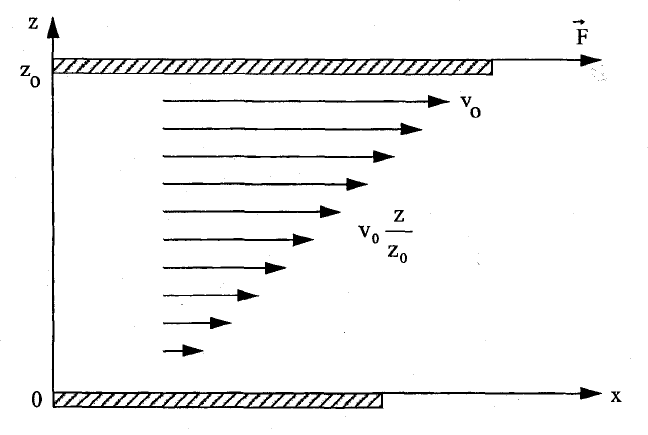
\includegraphics[width=0.7\textwidth]{img/figuur_1_theorie.png}
    \caption{Snelheidsverdeling in een viskeus midden tussen evenwijdige platen bij lage snelheden}
\end{figure}

Voor lage snelheden beweegt de vloeistof zich in lagen over elkaar. Dit heet \textbf{laminaire stroming}.
De laag $z = z_{0}$ heeft de snelheid $v_{0}$ de snelheid nul heeft. De snelheid van de 
vloeistoflagen daartussenin verandert lineair in functie van de hoogte z.
\\

$v = v_{0} \cdot \frac{z}{z_{0}}$ of $\frac{\delta v}{\delta z} = \frac{v_{0}}{z_{0}}$
\\

In het algemeen neemt de snelheid echter niet lineair toe met de dikte an de vloeistoflaag. 
De evenredigheidsconstante is ook afhankelijk van de aard van het flu\"idum, en wordt de
\textbf{viscositeitsco\"effici\"ent} genoemd. We bekomen de formule:
$$\frac{F_{W}}{S} = \eta \cdot \frac{dv}{dn}$$

Met
\\

$S=$ de oppervlakte van de vloeistoflagen

$n=$ de normaal loodrecht op dit oppervlak

$dv=$ de snelheidsverandering over de lengte

$dn=$ de normaal op S
\\

De \textbf{viscositeitsco\"effici\"ent} $\eta$ is dus de kracht per oppervlakte-eenheid nodig 
om snelheidsverschil van \'e\'en eenheid te handhaven tussen twee lagen vloeistof gelegen 
op een eenheidsfactor van elkaar.

\subsection{Laminaire stroming in een cilindervormige buis}

De wet van Hagen-Poiseuille geeft de snelheidsverdeling van de vloeistof 
in een horizontale cilindervormige buis bij stationaire, laminaire storming.
\\

$$v(r) = \frac{\pi(p_{1}-p_{2}) \cdot R^4}{4 \cdot L \cdot \eta}$$
\\
Het volumedebiet Q is het volume vloeistof dat per seconde door de buis stroomt.
Dit is te berekenen door die vergelijking over de doorsnede van de buis te integreren. 
Dit geeft: 
\\

$$\int_0^R2 \pi rdr \cdot v(r) = \frac{\pi(p_{1} - p_{2})\cdot R^4}{4 \cdot L \cdot \eta} $$
\\

Volgens de \textbf{wet van Poiseuille} is het debiet Q recht evenredig met het 
drukverschil $\delta p$ in het laminair regime. In een grafiek van Q in functie
van $\delta p$ geeft dit een rechte door de oorsprong; de richtingsco\"effici\"ent van de rechte is gelijk aan $\pi R^4 / 8\eta L$.
\\

\subsection{Overgang van laminair naar turbulent regime}

Als de snelheid echter te groot wordt, zal het laminair regime plaatsmaken voor een turbulent regime. 
Dit turbulente regime wordt gekenmerkt door wervelingen of draaikolkjes. Het hoogste
debiet waarbij de stroming nog juist stabiel laminair is, wordt het kritische debiet
$Q_{krit}$ genoemd.

\begin{figure}[h]
    \centering
    \caption{Overgang laminair naar turbulent regime}
    \label{fig:overgang_lam_turb}
    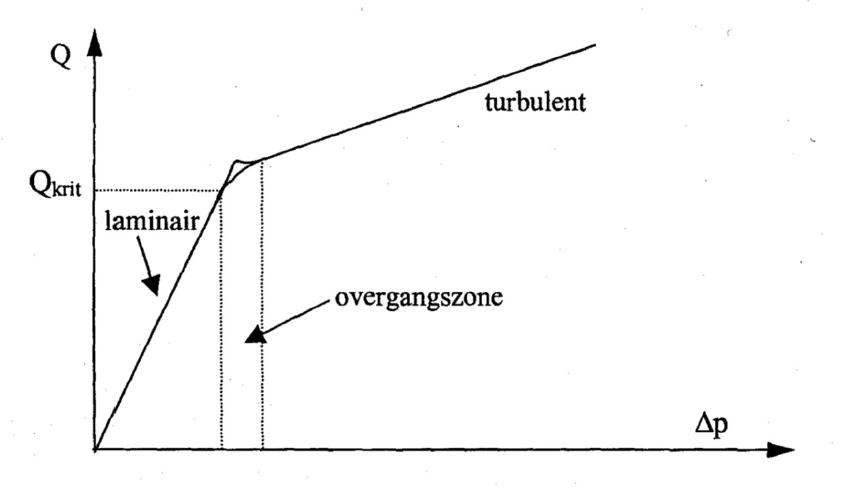
\includegraphics[width=0.7\textwidth]{img/figuur_3_theorie.png}
\end{figure}

Het is moeilijk om theoretisch te voorspellen bij welke stroomsnelheden laminaire
stroming zal overgaan in tubulente stroming. In dit kader speelt het 
\textbf{Reynoldgetal} een belangrijke rol.
\\

\subsection{Het Reynoldgetal}
De genormaliseerde gemiddelde stroomsnelheid $v/v_{0}$ wordt het Reynoldgetal genoemd:
\\

$$N_{R} = \frac{v \cdot \rho \cdot D}{\eta}$$
\\

Deze definitie geldt enkel voor een horizontale, cilindrische buis.
Voor andere systemen gelden andere definities.
\\

Het maximale Reynoldgetal waarbij de stroming nog juist stabiel is is ca. 2000.